\chapter{Pithos Design and Implementation}
\label{chp:DESIGN}

The generic state consistency model was presented in Section \ref{generic_event_update_model}. One of the key challenges that still remain was determined to be designing a root storage module specifically tailored to P2P MMVEs. The root storage model identifies in Section \ref{generic_event_update_model} includes the processes of state management and state persistency for the authoritative objects.

We've identified the main requirements of P2P MMVE state management and persistency in in Section \ref{key_challenges_cm} as: scalability,
reliability, fairness, responsiveness and security. In Chapter \ref{p2p_MMVE_state_persistency} it is argued that none of the current approaches to state persistency satisfy all identified requirements,

The focus of this thesis is, therefore exclusively on state management and persistency in P2P MMVEs. This chapter presents a design that satisfies all the identified requirements, along with implementation details and results.

Pithos, a novel hybrid multi-tiered state persistency architecture is
proposed. The novelty of Pithos lies in its support for both a responsive and a fair storage system, while also taking into account security aspects
of distributed storage. There are some storage systems that provide responsive or fair storage, but none that provide both. No storage system, designed specifically for P2P MMVEs, have taken security into account.

If Pithos is incorporated into an existing P2P MMVE consistency architecture, it will add the ability to handle both state management and state persistency. The addition of a robust state persistency mechanism, specifically designed for P2P MMVEs, will bring us one step closer to
the creation of a complete P2P MMVE architecture.
%%%%%%%%%%%%%%%%%%%%%%%%%%%%%%%%%%%%%%%%%%%%%%%%%%%%%%%%%%%%%%%%%%%%%%%

\section{Use cases and design goals}
\label{use_cases_goals}

The purpose of Pithos is to allow for efficient object storage and retrieval that satisfies all identified requirements. As is evident from root storage in the flow diagram in Figure \ref{fig_event_update_flowdiagram}, Pithos will interface directly with the VE logic, as well as receive updates from the update generator. For the purposes of this discussion, update generation is assumed to be part of game logic.

\begin{figure}[htbp]
 \centering
 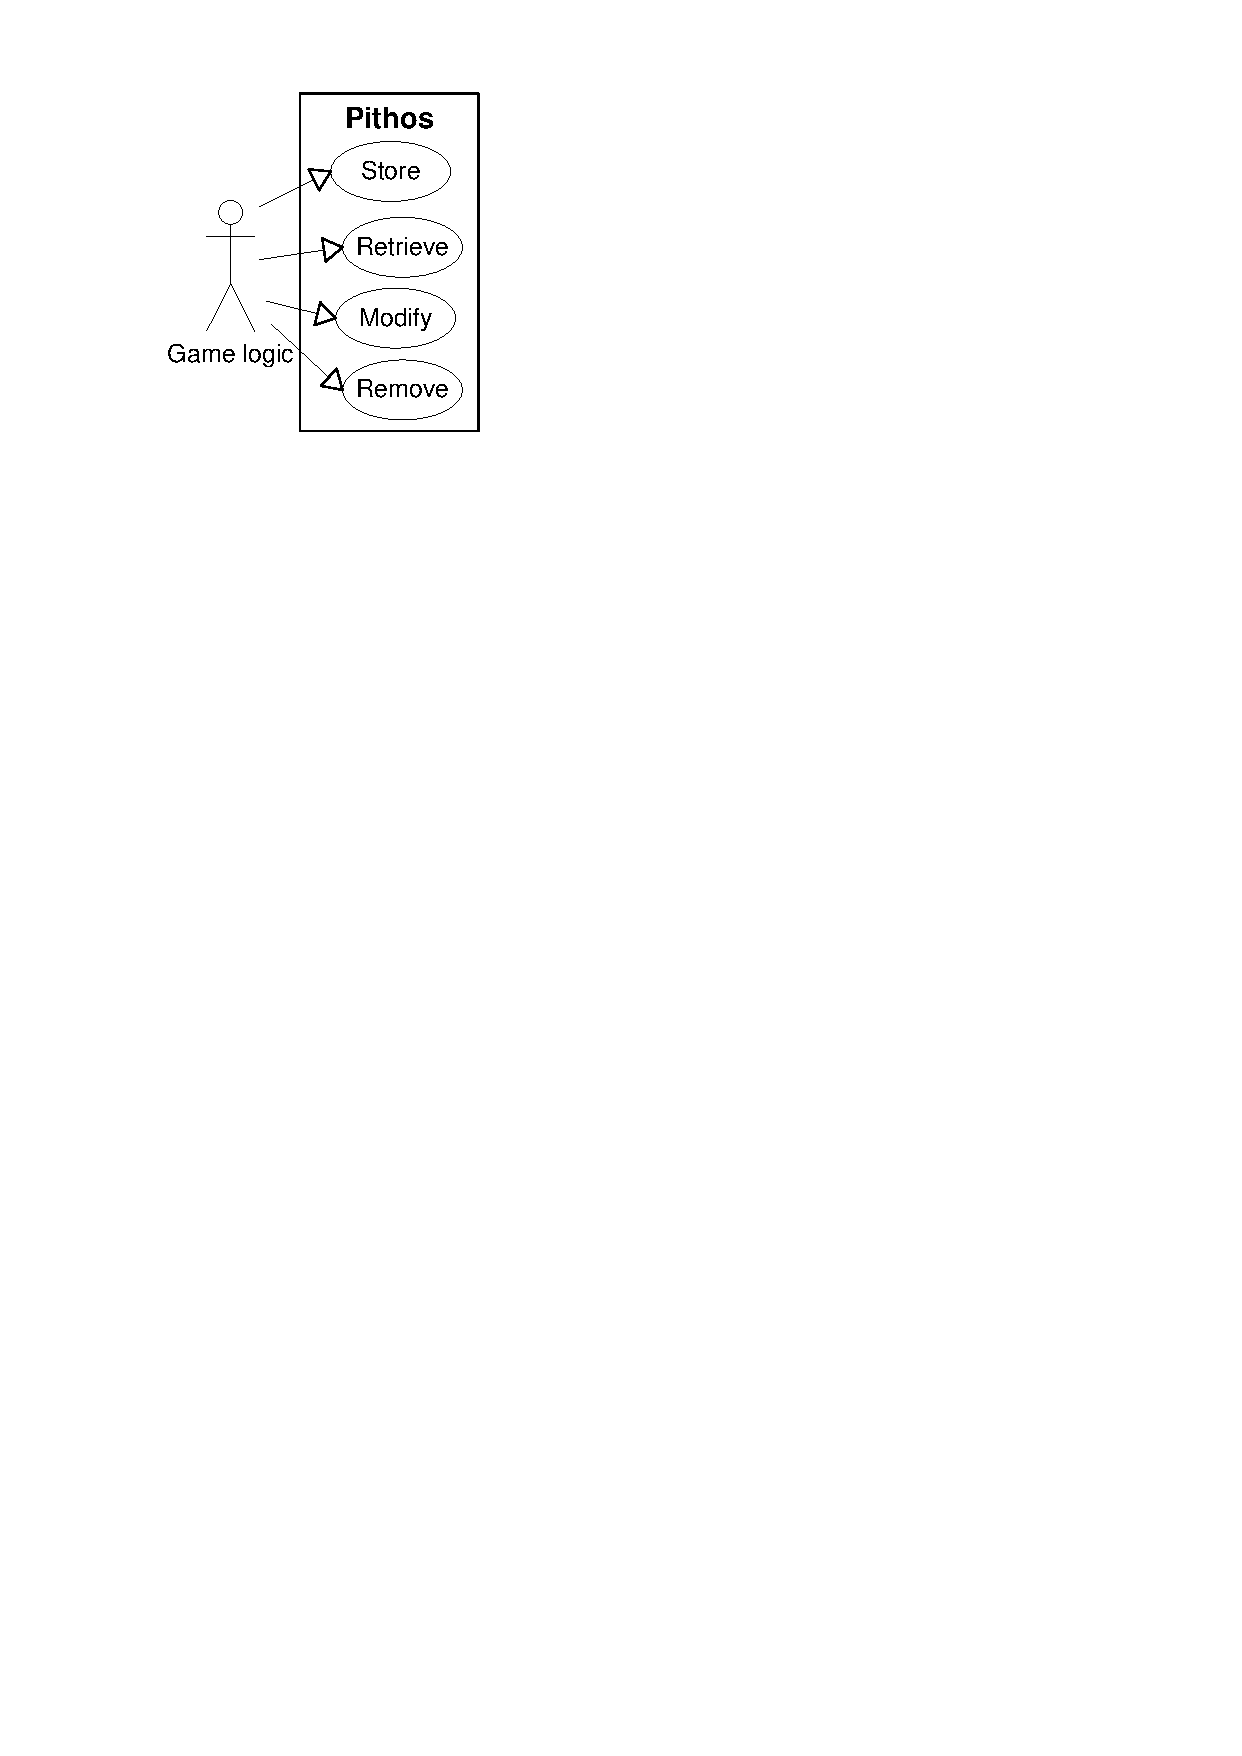
\includegraphics[clip=true, viewport=28mm 223mm 82mm 282mm, width=0.3\textwidth]{pithos_use_case}
 \caption{Use case diagram of Pithos}
 \label{fig_pithos_use_case}
\end{figure}

As shown in the use case diagram in Figure \ref{fig_pithos_use_case}, the VE logic should be able to use Pithos in four ways: store, retrieve, modify and remove. These are the use cases generally required of any storage system.

The VE logic will store data when a new object is added to the VE state. This can happen as a consequence of an event leading to the generation of a new object. An example of this is a rocket firing at a target. This event might generate a missile object to be sent towards the target.

Object retrieval will be required every time an event is received. The VE logic will retrieve the object state from memory, which is part of state management. Object states, other than the one being altered, might also be required by the logic to determine the effect an event will have, as discussed in Section \ref{event_logic_update}.

Object modification occurs every time an object update is generated. An object update, by definition, required a modification of the object state. Object removal might also be required to save storage space, although this is not essential to the correct functioning of the storage system.

Pithos is designed to fulfill all use case requirements as well as the requirements for P2P MMVE storage architectures as set out in Section \ref{key_challenges_cm}.

In order to fulfill the P2P MMVE storage requirements, the following design decisions were made:

The inspiration for Pithos come from two observations:
%
\begin{enumerate}
  \item One can combine multiple storage models and arrive at a model which possesses fewer disadvantages than any of the models used.
  \item Responsiveness is greatly increased in a fully distributed model, where there is no intermediate server that relays all information.
\end{enumerate}

Fully distributed architectures are, however, not scalable because the number of messages scaling by $O(N^2)$, where $N$ is the number of nodes in the network.

\section{Architecture}

\begin{figure}[htbp]
 \centering
 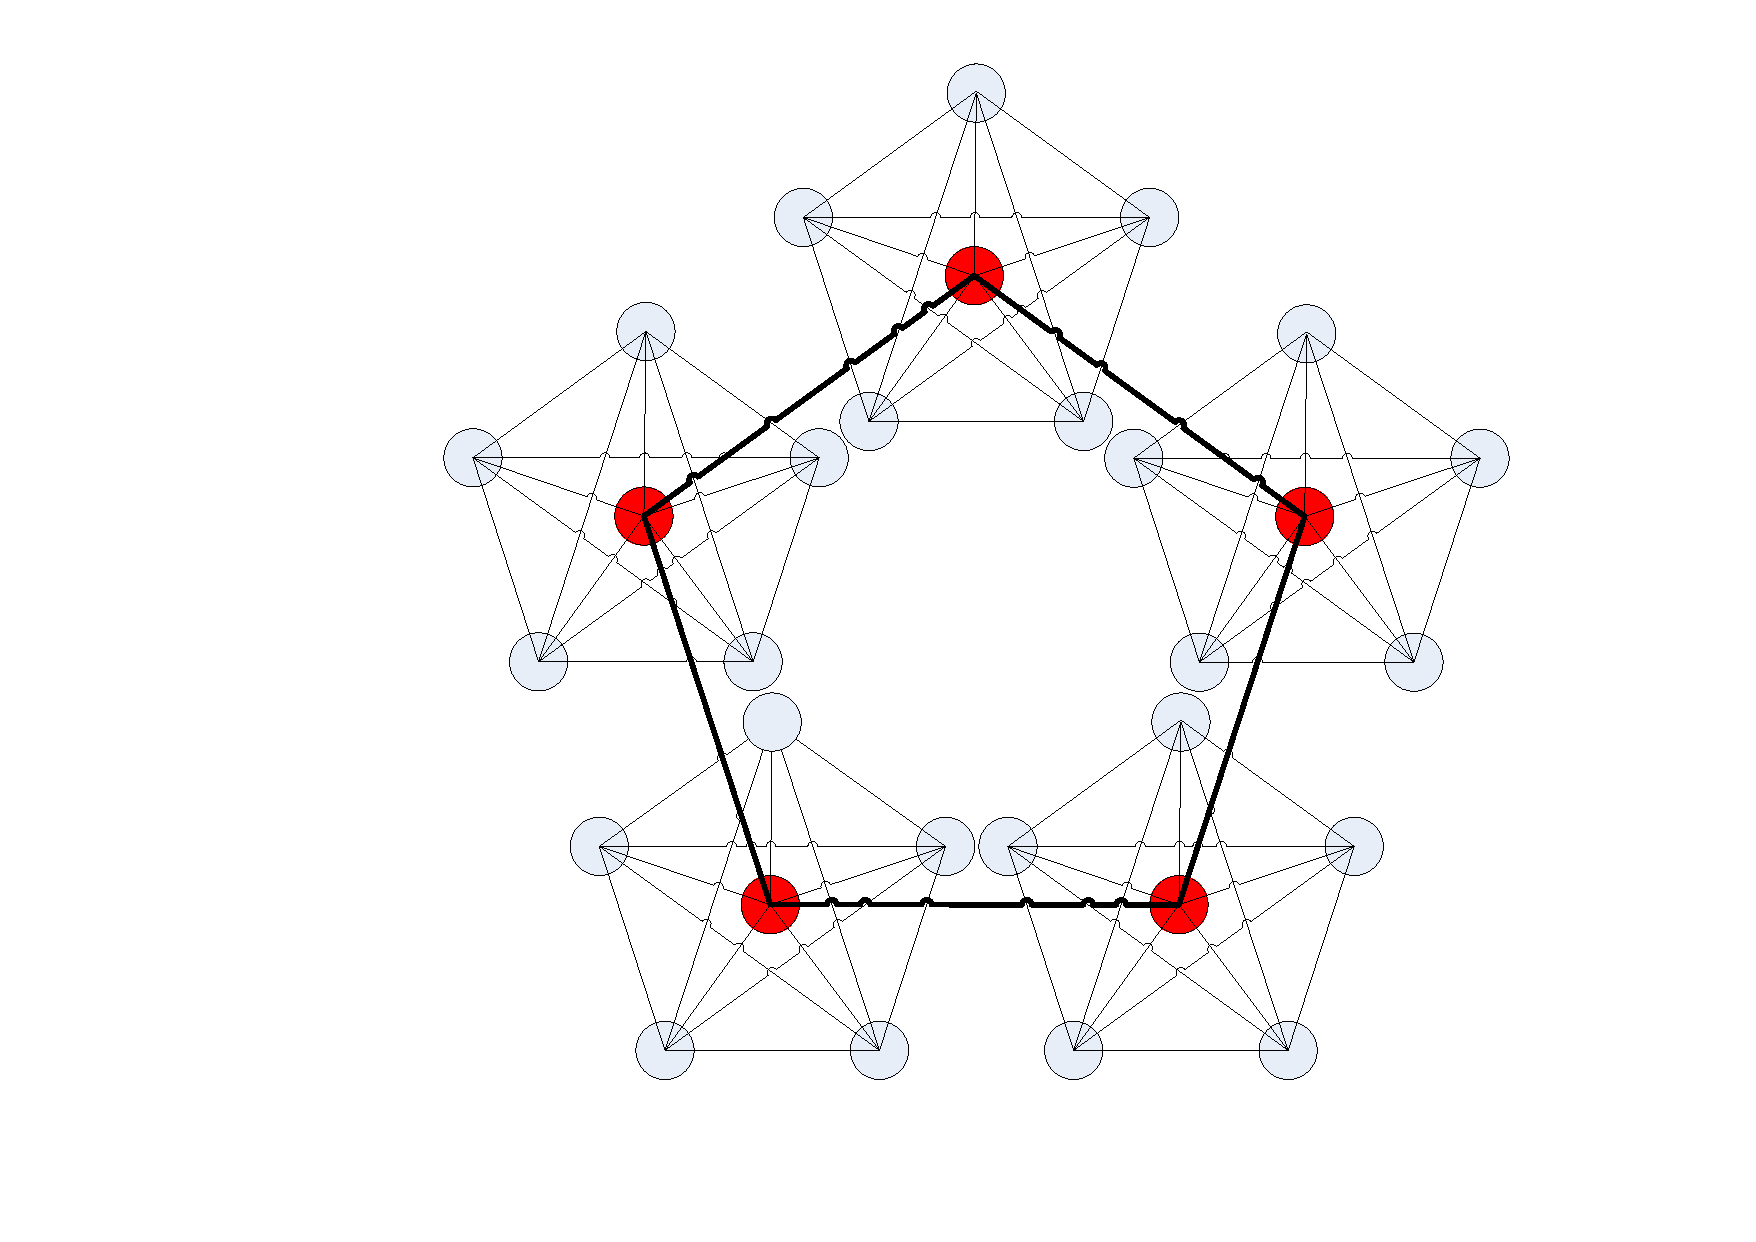
\includegraphics[clip=true, viewport=7.5cm 2.5cm 26cm 20cm, width=0.7\columnwidth]{CDHT_layout}
 \caption{Layout of the Pithos storage architecture}
 \label{fig_pithos}
\end{figure}
%
Figure \ref{fig_pithos} shows the Pithos architecture. The figure shows groups of fully connected peers (light blue and dark red), where all groups
are connected to each other in an P2P overlay through super peers (red).

Pithos groups peers to form a two tiered storage model. The first tier is a storage model at group level and the second is a storage model over all
groups. On the first tier, which is the intra-group level, a fully distributed storage system is used to allow for highly responsive read and write operations within the group. On the second tier, which is the inter-group level, a P2P overlay is used to store data between groups.

According to categorisation of \ref{storage_type_overview}, Pithos is a type of hybrid storage, that incorporates overlay storage and distance-based
storage. Responsiveness is achieved by constructing fully connected networks amongst groups of players and then storing objects that are mostly used
by the group within the group, as described in Sections \ref{grouping}, \ref{store_retrieve} and \ref{distance_based}. Reliability is achieved by
making use of replication and migration mechanisms as described in Section \ref{store_retrieve}. Security is achieved by using a certification
authority to assign node IDs and signing any storage and retrieve request with the requesting node's certificate, as described in Section
\ref{secure_ids}. Fairness is achieved by having all nodes store objects, as described in Sections \ref{store_retrieve} and \ref{distance_based}.

\subsection{Grouping}
\label{grouping}

%Speak more concretely of grouping algorithms
At the core of the architecture is the peer clustering mechanism. Two approaches are being evaluated: distributed clustering techniques (for example
affinity propagation \cite{affinity_propagation}) and dynamic regioning techniques (for example self-organising spatial publish subscribe (SOSPS)
\cite{self_organising_sps_post}).

\emph{Distributed peer clustering techniques}: make use of the flocking behaviour of players to dynamically group players into flocks or clusters
\cite{flocking}. The main idea of flocking is that players move around in groups, rather than randomly on their own. It is desirable that user
density within groups should remain constant, because a fully distributed architecture is not scalable. This means that groups should merge or split
as the user density within them change.

Affinity propagation clusters nodes using a similarity matrix to find similar nodes. The similarity matrix may contain user positions. In this case,
affinity propagation will group nodes depending on their location in a virtual world. This algorithm is ideally suited to P2P applications, since it
is a distributed clustering algorithm based on message passing.

\emph{Dynamic regioning}: divides the virtual world into regions that can be resized or further divided to maintain constant player densities across
regions. SOSPS creates dynamic regions based on a Voronoi overlay network \cite{voronoi_diagrams_survey}. Near constant user density is achieved by
increasing and decreasing the area sizes. This system is based on VON, a distributed Voronoi overlay network designed for MMVEs \cite{VON_VAST}.

\subsection{Replication}
\label{store_retrieve}

When storing objects in Pithos, replication is used to increase object availability under network churn and for security in the presence of malicious
nodes \cite{storage_and_chaching_PAST}. For every object that is stored in Pithos, $k$ object replicas are also stored. The number of replicas ($k$)
depends on the degree of network churn as well as the number of expected malicious users in the network. If the network churn is high, more replicas
are required to avoid the situation where all $k$ peers hosting an object leaves the network before any object migration can be done.

If a node leaves the network and stops to transmit ``keep alive'' messages, the migration mechanism will detect this and replicate the file on
another node. Replication exists intra- as well as inter-group and is useful in ensuring that if a nodes leaves the network, the data are not lost.
All object requests are routed to the peer with the next closest ID if the root peer leaves, because of how overly routing functions. The new
destination peers will possess the stored files, since Pithos stores overlay replicas at overlay neighbours.

Another reason to replicate game objects is to make the system more secure. If it is known that a certain percentage of users are malicious, it is
advantages to have more replicas than malicious users. This will allow for a secure system where object hashes can be compared to determine which
nodes are malicious and what version of an object is accurate.

\subsection{Distance-based storage}
\label{distance_based}

For Pithos to succeed as an MMVE storage architecture, intra-group data requests should be preferred to inter-group data requests. This requirement,
combined with the fact that the grouping algorithm geographically groups players in the virtual world, lends Pithos to a storage system based on
distance-based storage. Similar to interest management, the assumption is that players have a limited area of interest and require interaction with a
limited number of objects within range.

Therefore, distance-based storage is implemented on a group level rather than an individual level. This means that objects are stored on the nearest
group of players, rather than the nearest user. It is assumed that such an approach will alleviate the security and reliability challenges present in
distance-based storage \cite{gilmore_p2p_mmog_state_persistency}.

With group-based distance-based storage, it is assumed that because peers now store objects closest to the group, the objects that they are
interested in will most likely be stored within their own group. Therefore, most data requests should be intra-group requests. The overlay storage
component ensures that nodes that require data, which are not stored within their group, are still able to access requested data.

\subsection{Secure storage and node ID assignments}
\label{secure_ids}

In order to design a secure distributed storage system, one requirement for the P2P overlay is that nodes should not be able to select their own IDs
or it will not be possible to secure the system against attack. Node IDs should rather be assigned securely by some certification authority
\cite{secure_overlay_routing}.

To meet this requirement, Pithos implements its own certification authority to assign node IDs securely and promote security in the P2P overlay. A
certification server exists that handle ID requests from nodes. The server assigns IDs to nodes and provides the node with a signed certificate that
it may use to store data.

Whenever an object is stored or updated in the storage network, nodes have to sign the object to enable the tracking of object changes throughout the
life of the object. This system is very different from classic distributed file storage designs that advocate anonymity in storage. The fact that all
changes can be tracked to a specific node will simplify the task of eliminating user cheating.

\section{Oversim}

Pithos has been implemented in Oversim \cite{OverSim_2007}, a P2P simulation environment based in Omnet++, which allows for the measurement of identified requirements. Furthermore, it allows for the comparison of the current model with other state persistency models.

Oversim is a peer-to-peer and overlay network framework for the Omnet++ simulator. Oversim allows for the simulation of many well known structured or unstructured overlay protocols. It also allows for the development of applications that can use the already implemented overlays in a well defined architecture.

%Discuss the lack of documentation

    \subsection{Motivation}

To allow for greater control of the environment, as well as greater scale, it was decided to implement the first version of Pithos as a large scale network simulation. A simulation allows for careful selection of the environment parameters and tight control of the parameter values. This in turns allows one to keep all but one parameters constant and evaluate the effect of a design decision on the system for varying values of the free parameter.

The underlying Omnet++ simulation environment is a powerful network simulator in its own right. It allows for robust message and module definitions and contains many tools to assist with simulation measurement and monitoring.

Simulation also allows for greater scalability and simulating on a network with global Internet characteristics. Greater scalability is achieved, because thousands of nodes can easily be created, where all the nodes have global scale latency characteristics.

Implementing a large scale network application in the real-world would require thousands of computers spread across the globe. Such an environment will contain many variables out of the designer's control. Issues such as router congestion for example varies from day to day, which will produce varying latency results.

Because of these reasons, it was decided to first implement Pithos in simulation. This allows for the perfection of the design, under laboratory conditions, before the real world implementation is completed.

Pithos is intended for future real world implementation, however, so all modules created were written in such a manner to allow for easy porting. No tasks that are performed in Pithos make use of any simulation ``short cuts'', such as accessing the global peer list. Only statistics gathering modules are allowed to make use of these simulation features.


    \subsection{Underlay network}

At the base of an Oversim simulation is the underlay network. The underlay network determines the types of nodes in the Oversim simulation. Three underlay types exist: the ``simple'', ``INET'' and ``SingleHost'' underlays \cite{oversim_applications}.

In the simple underlay, node latencies are determined by the distance between nodes placed in an $n$-dimensional Euclidean space. The positions of the nodes are chosen to match the latencies of the CAIDA/Skitter project. Different nodes are also assigned different bandwidth and jitter parameters to simulate a heterogenous network. The simple underlay, therefore, captures the delay characteristics of a global scale network in an abstract way. The simple underlay network is ideal for simulating large scale overlay networks because of its simplicity and high accuracy.

The INET underlay is based on the Omnet++ INET underlay and allows for the simulation of the complete IP level stack. This includes backbone routers and gateways. It also contains many implemented MAC layer protocols. The INET underlay is well suited to simulating lower level communication protocols or wireless protocols such as IEEE 802.11 (Wi-Fi).

The SingleHost underlay allows for interaction with a physical network. It allows for the implementation of physical nodes, running on networks computers. These physical nodes can then connect to a simulated network and receive packets with bandwidth and delay characteristics as if they were situated on a network with the simulation's specific characteristics.

To be able to simulate Pithos for the large numbers of nodes required, as discussed in Section \ref{scalability_req}, it runs on the simple underlay. Pithos is dependant on the delay characteristics of the lower level protocols, but the CAIDA and Skitter measurements capture these quantities in their measurements. The reasons for different delay characteristics in the network is not required.

\begin{figure}[htbp]
 \centering
 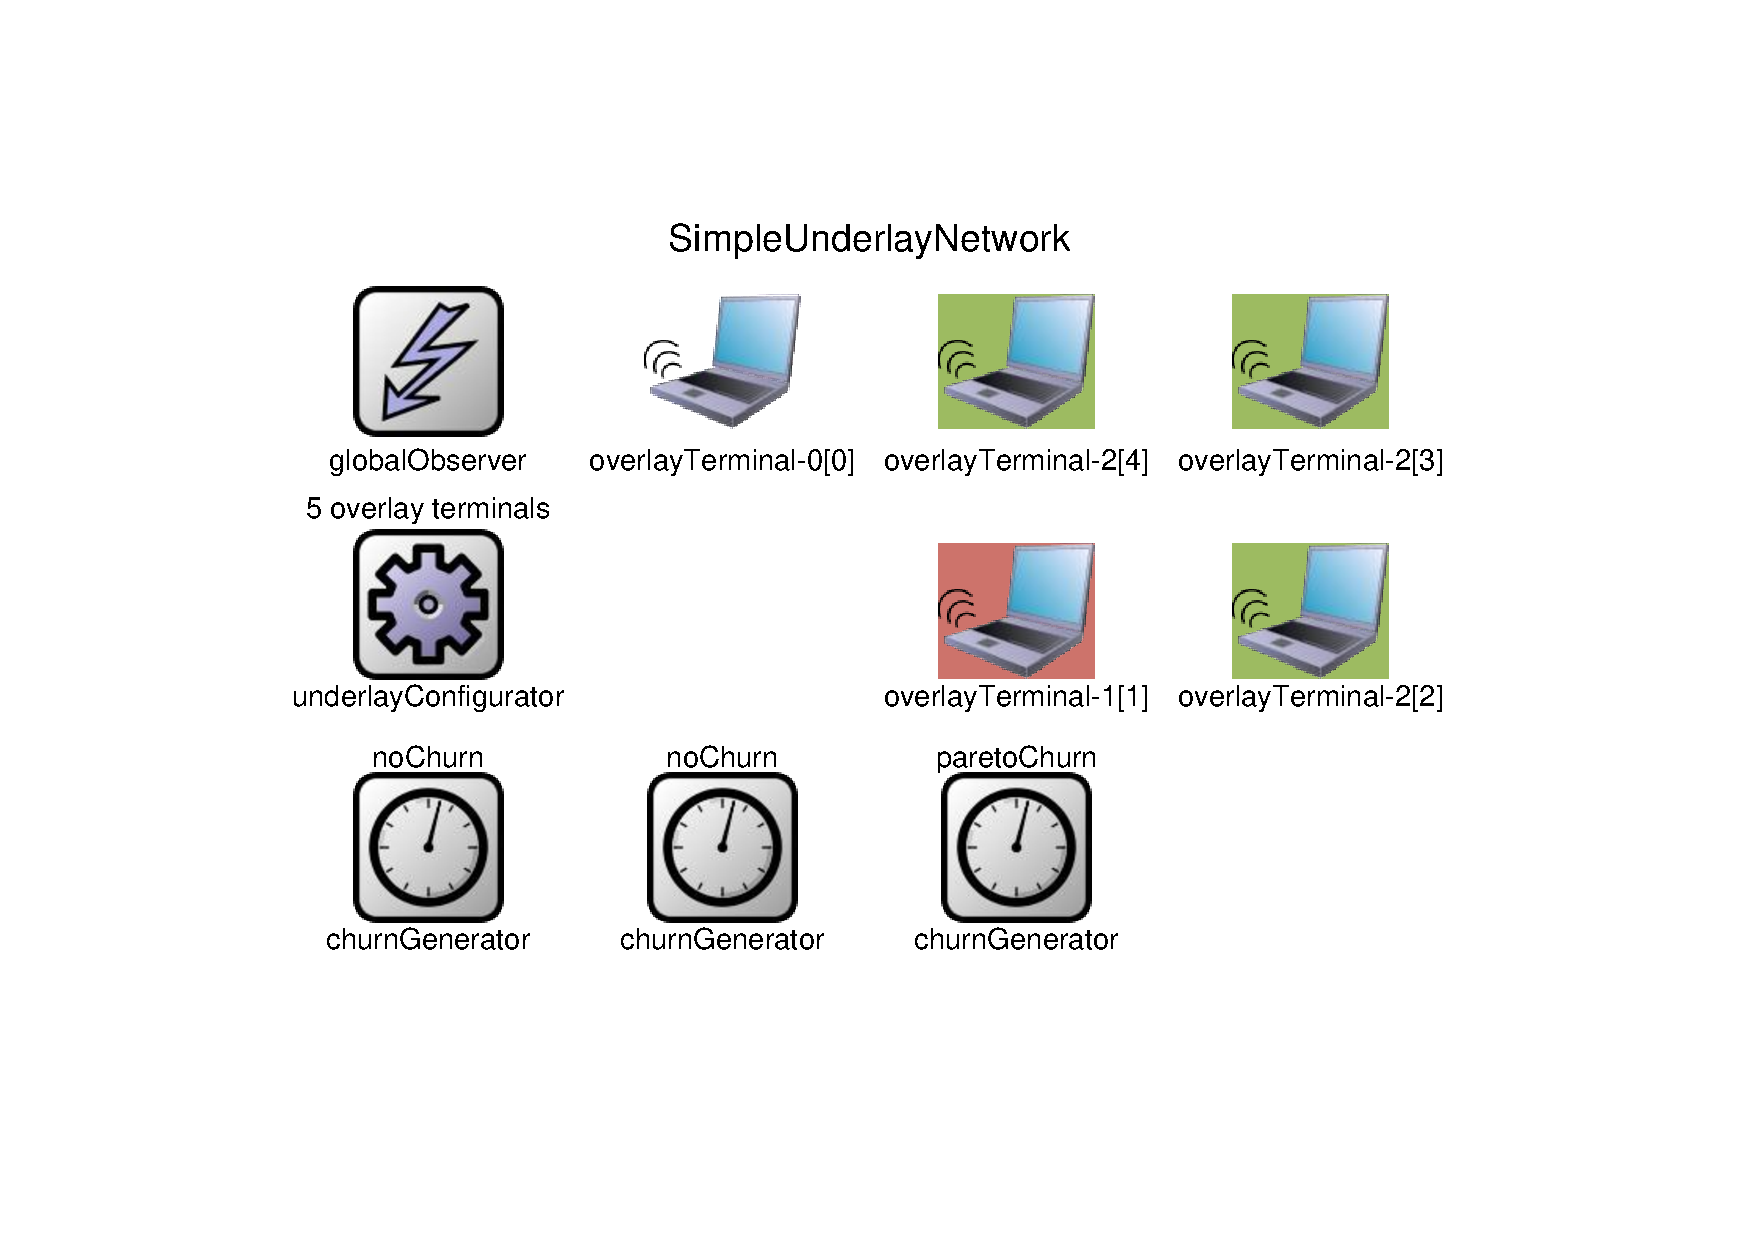
\includegraphics[clip=true, viewport=49mm 48mm 245mm 173mm, width=0.5\columnwidth]{Oversim_terminals}
 \caption{The Oversim simple underlay network with the three Pithos terminal types}
 \label{fig_oversim_terminals}
\end{figure}

Figure \ref{fig_oversim_terminals} shows the Pithos simple underlay network after the first five nodes have been generated. Each overlay terminal is an Oversim node containing its own protocol stack. The underlay configurator is responsible for setting up the network. The global observer contains the global node list, global statistics and parameters modules. It is used to generate global statistics and by the lower levels to keep track of all nodes.

Three churn generators also exist, one for generating each of the three Pithos node types. Churn generators model users joining and leaving the network. There are three types of churn generators: ``no churn'', ``lifetime churn'' and ``Pareto churn''. The ``no churn'' churn generator creates nodes every specified number of seconds until a specified number of nodes are reached and does nothing further. This generator can be used to test simple networks, where churn is not an issue, or for initial testing of the first prototype.

Lifetime churn creates nodes with specified average lifetimes, sampled from an exponential distribution. This is a distribution regularly used to model lifetimes in reliability engineering. Pareto churn samples node lifetimes from a Pareto distribution, instead of an exponential distribution. This churn generator type requires mean node lifetime as well as mean node dead time to be specified.

A node type is determined by the protocols executing on every layer of the Oversim architecture. The Pithos node types will be explained in Section \ref{pithos_node_types}.

    \subsection{Node architecture}

\begin{figure}[htbp]
 \centering
 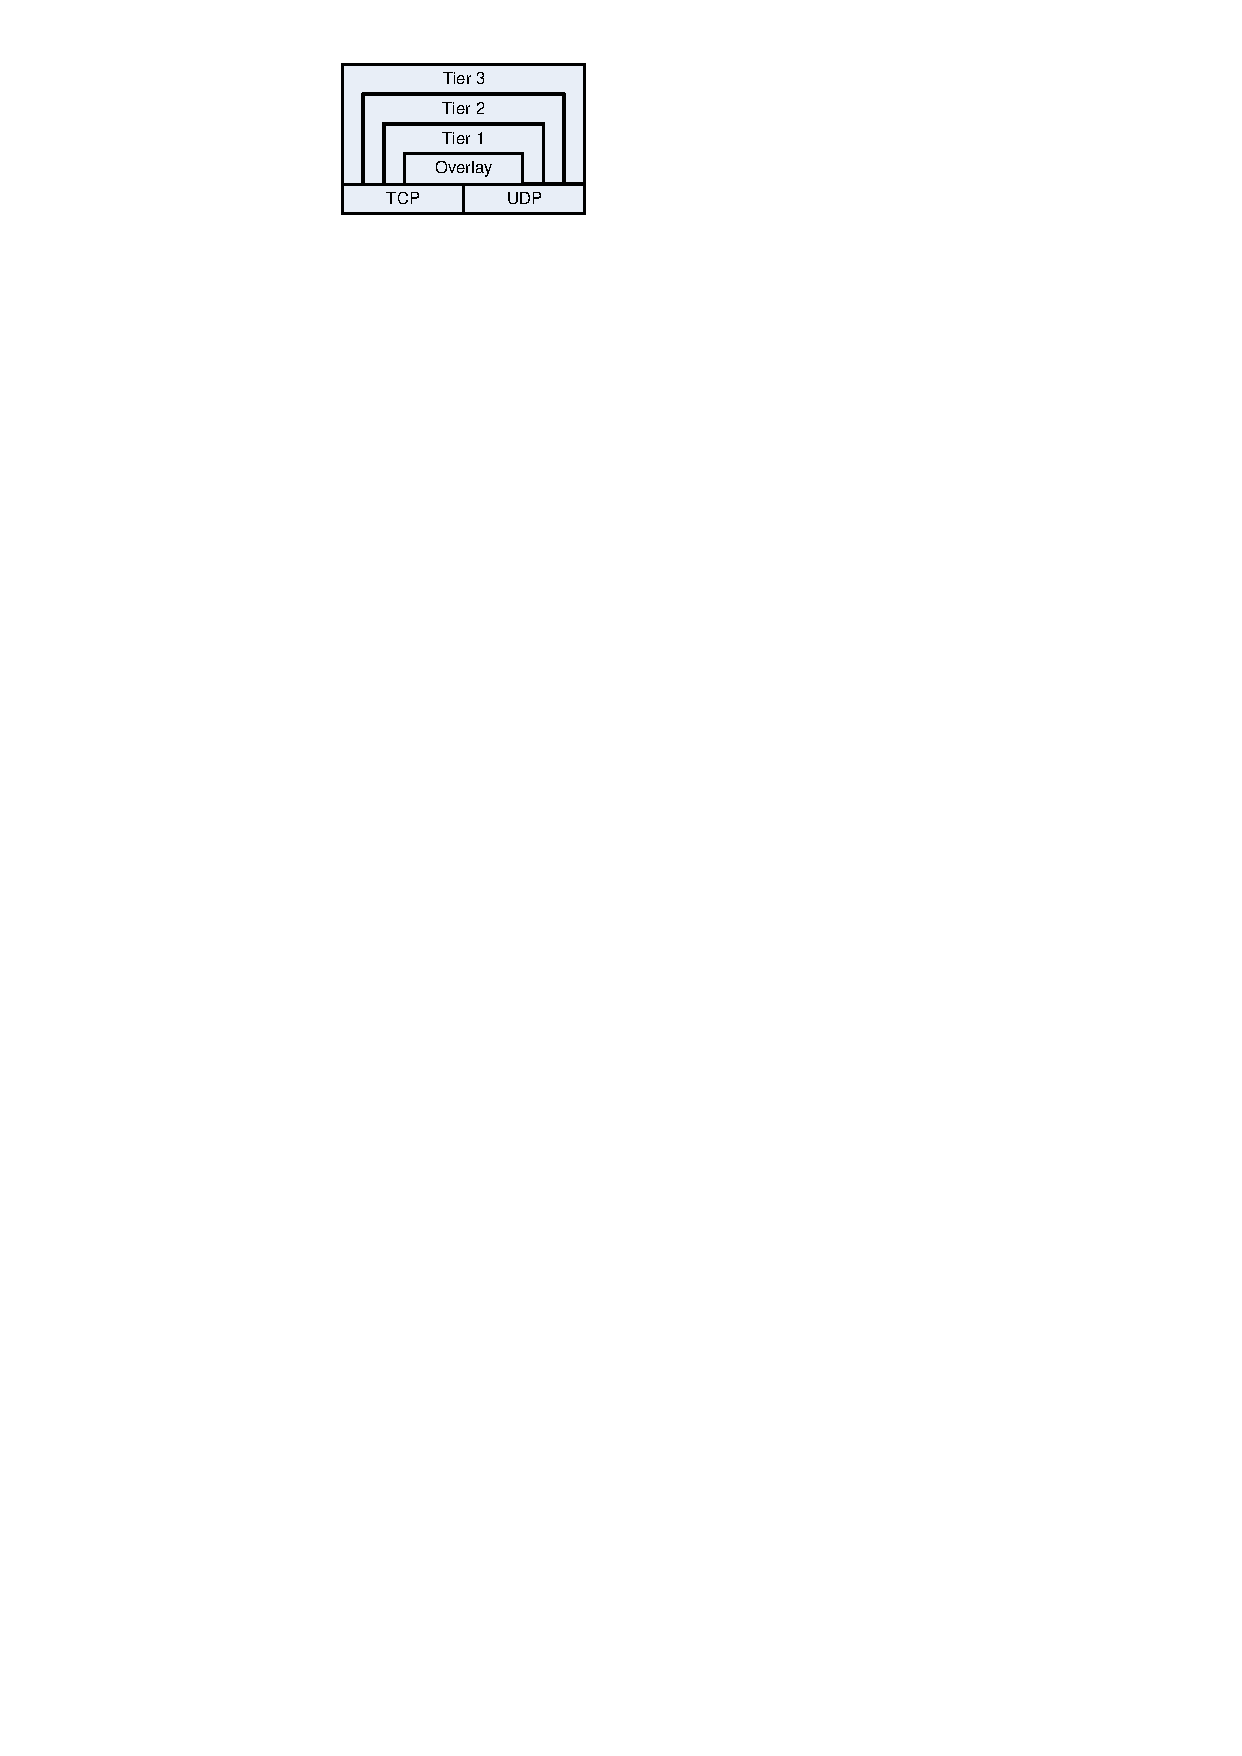
\includegraphics[clip=true, viewport=57mm 260mm 100mm 287mm, width=0.5\columnwidth]{Oversim_layers}
 \caption{Oversim node architecture layers}
 \label{fig_oversim_layers}
\end{figure}

%Also show the Oversim picture

Every node in Oversim contains a layered architecture, as shown in Figure \ref{fig_oversim_layers}. The Oversim node architecture contains the layers: TCP, UDP, Overlay, Tier 1, Tier 2 and Tier 3.

The transport control protocol (TCP) and user datagram protocol (UDP) are both transport level protocols, according to the OSI protocol stack specification. These two layers are the lowest communications layers in Oversim and allows message passing to other nodes.

The overlay layer is where the P2P overlay is housed. This can be any of the well known structured or unstructured overlays, such as Pastry, Chord or Gia. The three tiers above the overlay layer are the application level layers and is where application that use an overlay may be implemented. Three application layers are allowed.

Tier 1 can communicate with the Tier 2, overlay, TCP and UDP layers. Tier 2 can communicate with the Tier 1, Tier 3, TCP and UDP layers. Tier 3 can communicate with the Tier 2, TCP and UDP layers. Internal communications are usually between tiers and TCP and UDP communication occurs when a layer wishes to send a message to the same layer on a different node.

\begin{figure}[htbp]
 \centering
 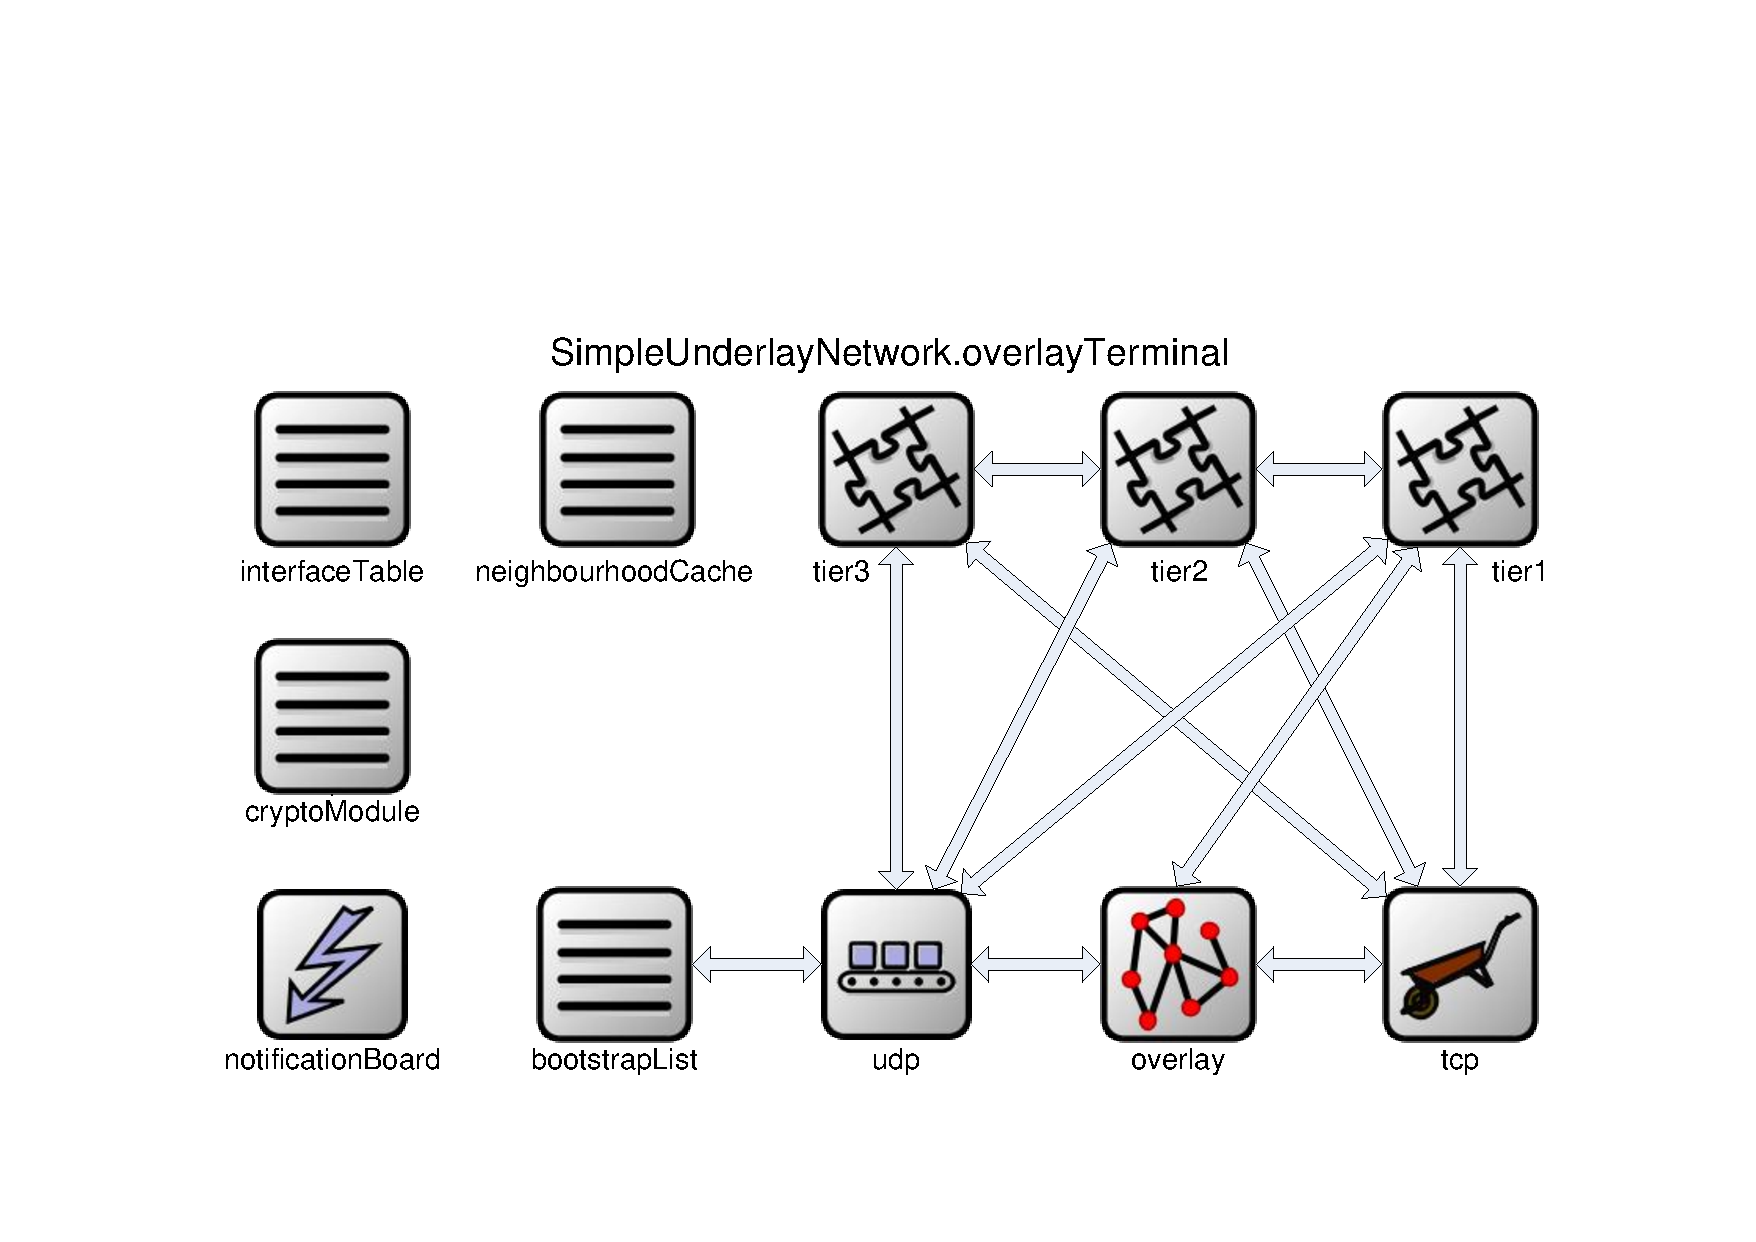
\includegraphics[clip=true, viewport=33mm 27mm 262mm 197mm, width=\columnwidth]{Oversim_architecture}
 \caption{The components of an Oversim terminal, including the tiered node architecture.}
 \label{fig_oversim_architecture}
\end{figure}

Figure \ref{fig_oversim_architecture} shows the complete Oversim node architecture. The tiers, udp, tcp and overlay are connected as explained earlier. UDP is also connected to a bootstrap list module, which assists nodes with joining the UDP network. The neighbourhood cache, interface table, crypto module and notification board modules are also present, but these modules are unused in Pithos.

    \subsection{Generic consistency extension}
    \label{generic_consistency_extension}

%Show the generic consistency architecture in Oversim

To allow Oversim to simulate a complete consistency architecture, the Oversim framework itself was extended. The three tiers were replaced with all the elements identified in the generic consistency model in Section \ref{generic_event_update_model}. Practically, this required the implementation of a new type of overlay terminal type, replacing the tiers with the following layers: agent, event layer IM, event dissemination, event ordering, game logic, root object updater, root object store, update layer IM, update dissemination, object merger, local object updater, local object store, display updater, overlay Storage.

Every new layer can communicate with the layer above and below it, and can also communicate with its version on another node using UDP or TCP. This allows for the consistency model to be distributed amongst any number of nodes. A module can either send its information to the layer below it within the same node, or it can send it to the layer below it on another node.

Every module can contain a collection of sub-modules which implements the layer itself. It the layer is not implemented, a dummy layer may be specified. The Pithos implementation is located within the root object store module. An application that provides Pithos with test inputs called ``PithosTestApp'' is situated within the root object updater layer. Pithos also makes use of overlay storage, which is implemented in the overlay storage module. Overlay storage requires a P2P overlay for routing purposes, which is why it is connected to the overlay layer.

\section{Pithos implementation}

Pithos is implemented in the root object store layer of the generic consistency model in the extended Oversim architecture.

\subsection{Node types}
\label{pithos_node_types}

On a network level, Pithos consists out of three node types: super peers, peers and a directory server.

The single directory server, which is a normal three-tiered Oversim node, places joining peers into groups represented by super peers. The directory server allows peers to join the network (Section \ref{network_join_iplementation}) and be placed into groups (Section \ref{network_join_implementation}).

Super peers represent and manage groups. All the functionality of the super peer is implemented by the super peer logic module. Peers handle requests from the higher application layers and consist out of the peer logic, ledgers, DHT storage and group storage modules.

It is possible for a single Pithos terminal to be both a peer and a super peer. In that case, it contains all modules of both the super peer and peer node types.

\subsection{Module types}
\label{pithos_module_types}

\begin{figure}[htbp]
 \centering
 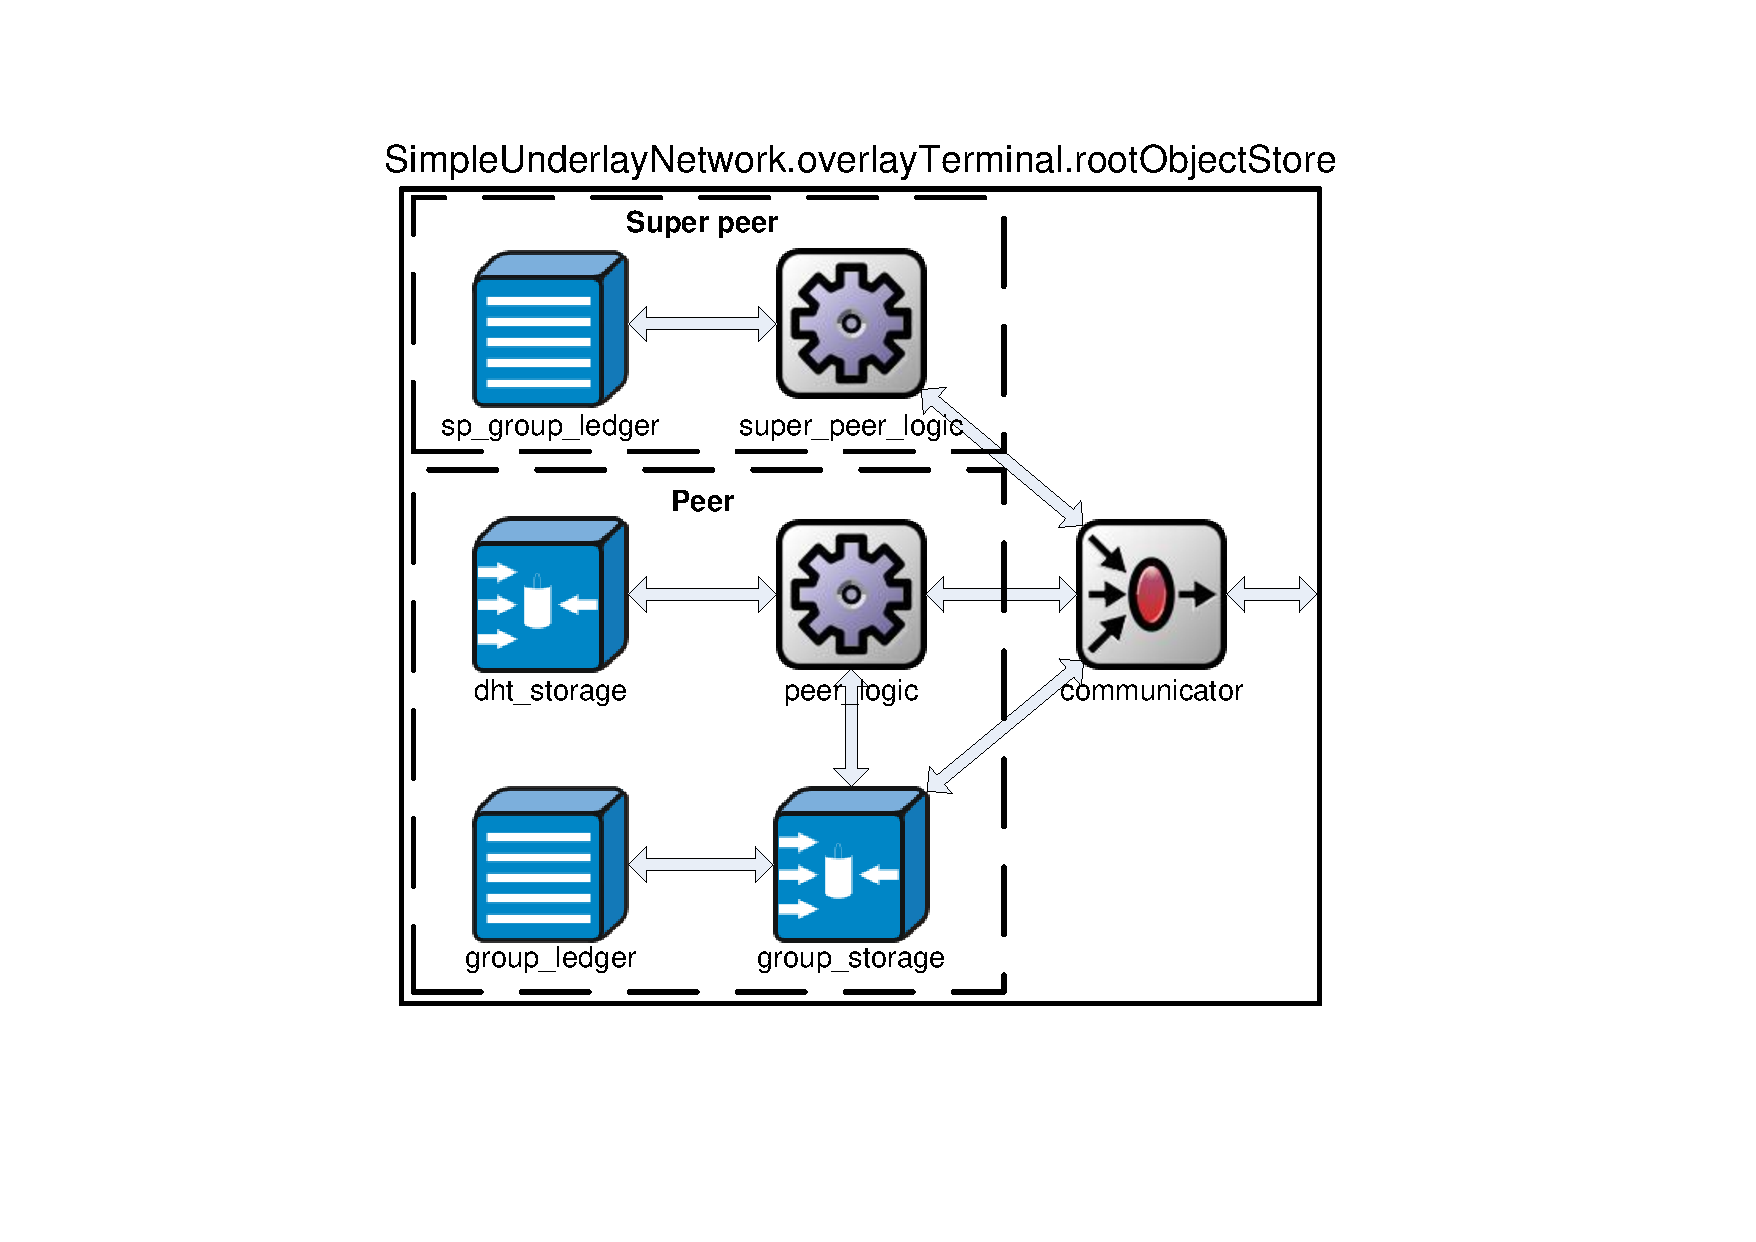
\includegraphics[clip=true, viewport=64mm 39mm 227mm 186mm, width=0.5\columnwidth]{Oversim_root_object_store}
 \caption{Pithos super peer and peer modules in Oversim}
 \label{fig_oversim_root_object_store}
\end{figure}
%
Figure \ref{fig_oversim_root_object_store} shows the Pithos modules related to the super peer and peer module types. The figure is divided into three sections: Super peer, peer and communicator.

\subsubsection{Communicator}

A simple module in Omnet++ is a module that implements a C++ class. All modules in Figure \ref{fig_oversim_root_object_store} are simple modules. Compound modules also exist that are combinations of simple modules, where the simple modules are connected to each other and external gates in some way.

Oversim requires a single simple module to be of type: ``BaseApp''. Oversim delivers messages from the layers above and below a layer to the module extending the BaseApp module. This means that because of Oversim's architecture, all message must go through a single module. When Pithos was designed, it was decided that placing all functionality in a single module would be a bad design decision. A single module would not allow for a modular implementation and would make future extensions more difficult.

The communicator module was then created, which received and sent all communications to the upper and lower layers. All message received or sent are, therefore, routed through the communicator module. The design of the communicator module was done to make it as transparent as possible. Another function of the communicator module was outbound message verification. The communicator module ensures that all messages sent contains a destination IP address, source IP address and type.

Transparency was achieved by designating certain gates for certain types of traffic. If a message is received on a gate with a specific purpose, that message is processed in a way consistent with that purpose and then transmitted. This design allows other modules to be expanded with new message types. Those message then only have to be sent to the correct gate to ensure correct handling of the message. The addition of a new message type, therefore, rarely required alterations to the communicator module.

\subsubsection{Super peer logic}
\label{pithos_module_types_sp_logic}

The super peer logic module implements all the functionality of the super peer node, except for keeping track of group objects. The tasks of the super peer logic include handling joining peers, ensuring group consistency (Section \ref{group_migration_implementation}), initiating object repair (Section \ref{object_implementation_implementation}) and maintaining a list of group objects and on which peers those objects are stored (Section \ref{pithos_module_types_ledgers}).

\subsubsection{Peer logic}

Peer logic
\begin{enumerate}
  \item  receives all store (Section \ref{store_implementation}), retrieve (Section \ref{retrieve_implementation}) and modify (Section \ref{modify_implementation}) requests from the higher application layer,
  \item forwards those requests to the required modules,
  \item forwards responses received from modules to the higher layer,
  \item keeps track of all outstanding requests (Section \ref{pending_rpcs_implementation}), and
  \item verifies received data from multiple sources for added security (Section \ref{object_verification_implementation}).
\end{enumerate}

\subsubsection{DHT storage}

The DHT storage module forms part of the peer node. The DHT storage modules interfaces with the overlay storage module on behalf of the peer. The DHT storage module received requests from the peer logic modules for overlay storage services. The DHT storage module also keeps track of all outstanding overlay storage requests.

In the Oversim simulation, the DHT storage module interfaces with Oversim's DHT implementation, written by Gregoire Menuel and Ingmar Baumgart. The DHT implementation itself is located in the overlay storage module of the extended Oversim node architecture that represents the generic consistency model, as described in Section \ref{generic_consistency_extension}.

The Oversim DHT implementation contains data structures to store data, route requests via the overlay to other DHT modules and allows peers to join a network wide overlay. It supports put, get and modify requests. The Oversim DHT implementation meets all Pithos's overlay storage requirements and is able to run on any of the overlay implemented in Pithos.

\subsubsection{Group storage}

The group storage module forms part of the peer node. It receives requests from the peer logic module for group storage services. The group storage module
\begin{enumerate}
  \item handles group store, retrieve and modify requests from the peer logic,
  \item maintains a view of all peers currently in the group,
  \item maintains an object store where it stores some subset of the group objects,
  \item is responsible for the administration of group membership on behalf of the peer,
  \item monitors the availability of group peers and informs the the super peer of peers that left the group,
  \item informs the group of new object stored, and
  \item repairs objects if requested to do so by the super peer.
\end{enumerate}

\subsubsection{Ledgers}
\label{pithos_module_types_ledgers}

Each peer and super peer in the network contains a group ledger. The group ledger is an abstract data type that maintains lists of all objects stored in the group, as well as all peers that are part of the group. The group ledger is used by the group logic and super peer logic modules to keep track of all group objects and peers. The group ledger is required whenever an object is retrieved within the group.

The group ledger was designed for efficient storage, while still allowing high speed access to data. In order for the ledger to be efficient, it implements a map of object ledgers, where each object ledger contains object information and a list of peers where that object is stored on. The group ledger also contains a peer ledger list, where each peer ledger contains a list of objects that are housed on that peer.

In the object ledger, each entry in the peer list is a reference to peer information contained in the peer ledger. In the peer ledger, each entry in the object list is a reference to peer information contained in the object ledger. This means that peer and object information are only stored once, and always referred to by references. This dually linked structure allows for searching in any direction. Objects are stored in a map, since there might be thousands of objects in a group, compared to tens of peers. Efficient object lookup is, therefore, a priority, whereas sequential peer search is sufficient.

\subsection{Key mechanisms}

While the previous section describes the static structure of the Pithos implementation, this section will describe the key mechanisms present in Pithos to achieve the desired design goals specified in Section \ref{use_cases_goals}. The purpose of each mechanism will be described along with how it has been implemented in Pithos with reference to the modules present.

    \subsubsection{Joining the network and grouping}
    \label{network_join_implementation}

    The first task of a Pithos peer is to join the network and a group. This is done using the directory server, which possesses a static IP address and port that is known to every new peer and super peer. Whenever a super peer is created or potentially selected, it advertises its information with the directory server. This information includes its IP address, port and location of the super peer.

    For simulation purposes, each super peer is assigned a random location created by sampling both an x and a y coordinate from a uniform random distribution. What this would mean practically is that super peers have some assigned region they control. Joining peers are assigned positions in the same uniform random manner when they are initialised. When a peer wishes to join the network and a group, it queries the directory server, supplying its own position. The directory server then replies to the joining peer with the IP and port of a super peer that is closest to it.

    The joining peer then sends the same type of join request to the supplied super peer address. The super peer can then elect to accept or reject the joining peer. This extra step is intended to prevent groups from becoming overloaded. The super peer can supply an alternative address for the joining peer to contact. This extra step is also intended to compensate for the movement of super peers. If super peers move and by the time a joining peer contacts a super peer there is another super peer in closer range, the super receiving the join request can supply the joining peer with the address of the closer super peer.

    If the super peer accepts the joining peer, it sends that peer a list of all peers currently in the group, as well as a list of objects currently available in the group. The super peer also informs all other group peers of the newly joined peer.

    The directory server might become overloaded when tens of thousands of nodes are present, although this has never happened in simulation. The grouping algorithm will be improved by implementing it in a distributed fashion. The current implementation is, however, sufficient for the purposes of this study, where a focus is placed on improving distributed storage for P2P MMVEs, after users have been placed in groups. Much research has been performed on distributed grouping algorithms, as reviewed in Section \ref{grouping}, and it is believed that using one of those methods, or a modified version thereof, in the eventual implementation will be sufficient.

    \subsubsection{Storing data}
    \label{store_implementation}

    Store requests are received from the higher level PithosTestApp, described in Section \ref{pithostestapp}. Figure \ref{fig_pithos_msg_flow_store} shows the message flow between all Pithos modules for an object store request.

\begin{figure}[htbp]
 \centering
 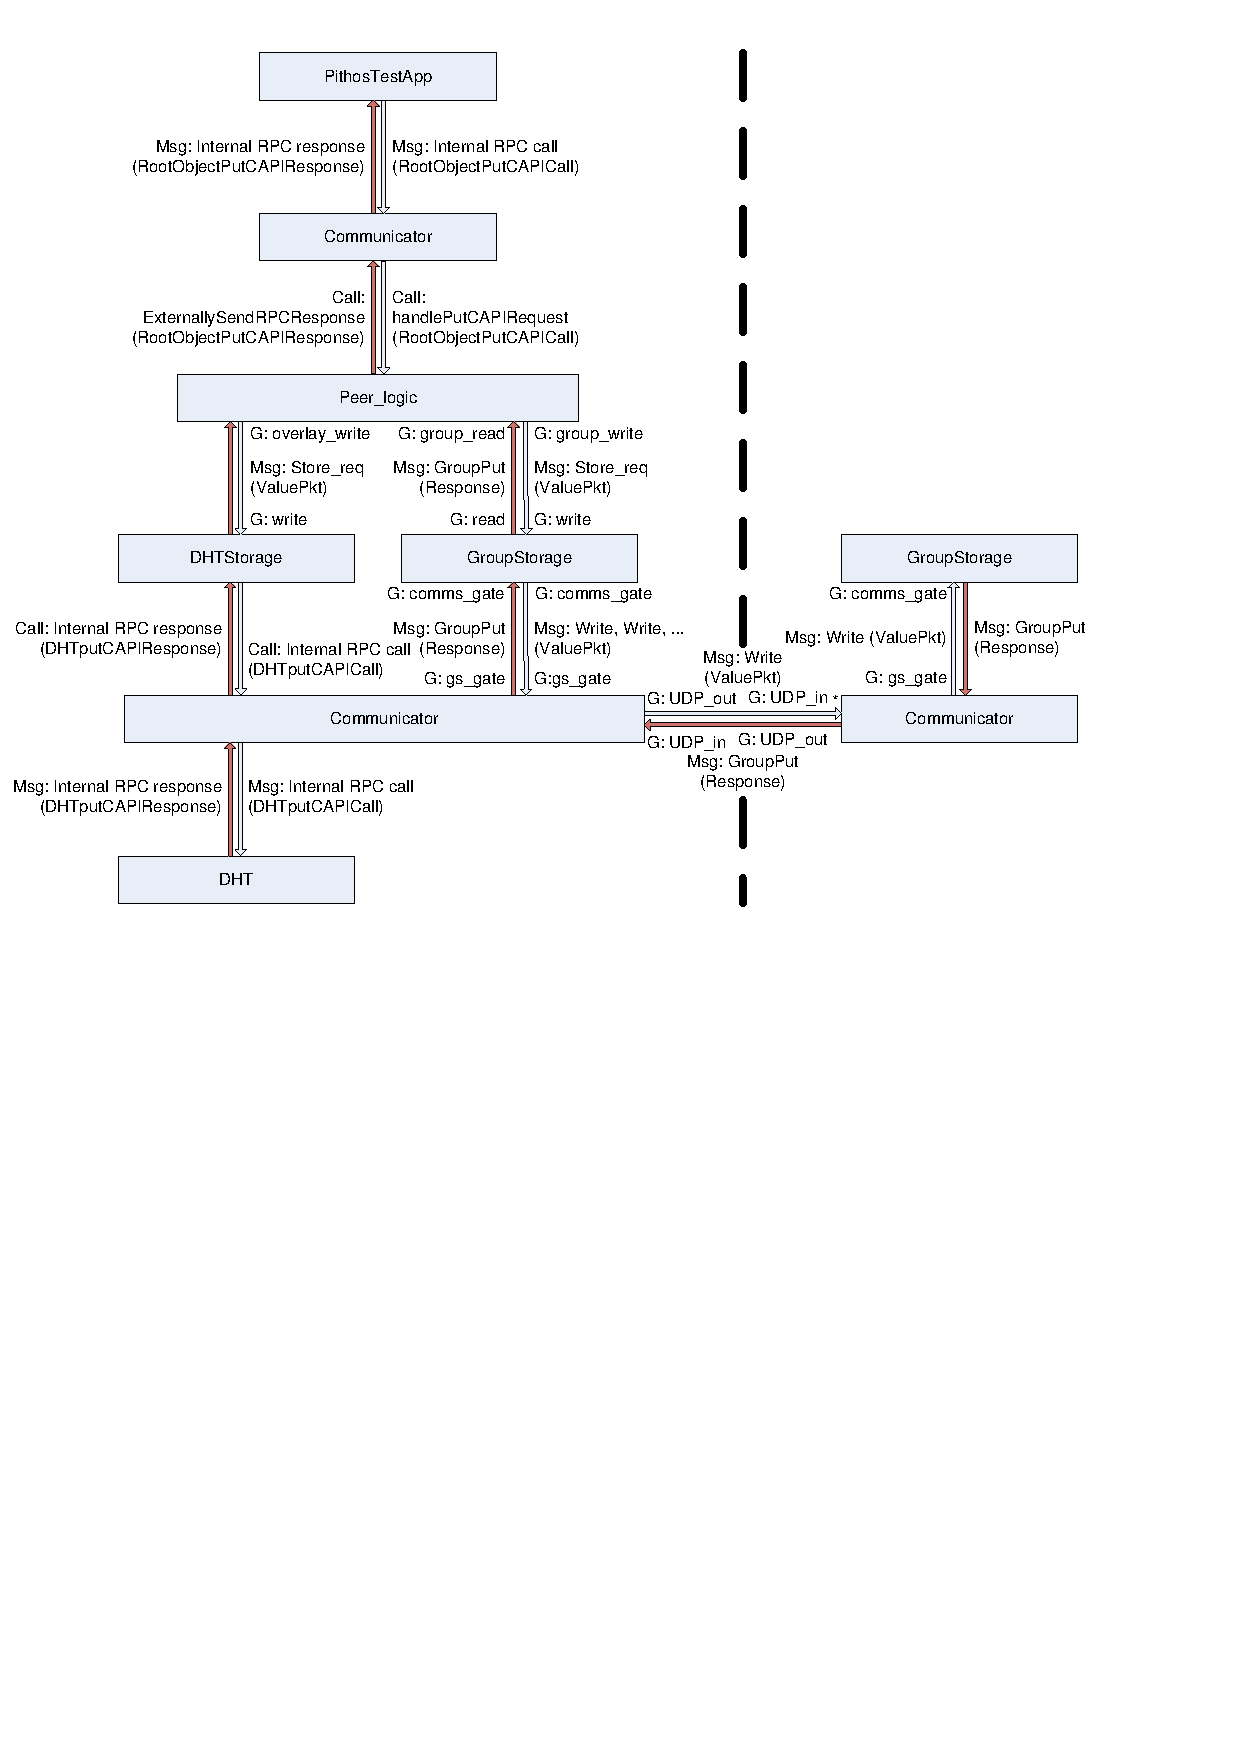
\includegraphics[clip=true, viewport=2mm 143mm 185mm 289mm, width=\columnwidth]{Pithos_msg_flows_store}
 \caption{Pithos message flow as a response to a store request}
 \label{fig_pithos_msg_flow_store}
\end{figure}

Within the same node, the PithosTestApp sends a remote procedure call (RPC) to the Pithos communicator module, containing the object to be stored. The communicator forwards all requests from PithosTestApp to the peer logic module. The peer logic module creates a store request message which it sends to both the DHT storage and group storage modules. This is the request from peer logic to the two modules to store the object in both the DHT and group storage. The DHT storage module translates the storage request message into another RPC, which is understood by the DHT module. The internal RPC call is sent to the DHT module via the communicator. The DHT module further handles overlay storage and returns an internal RPC response indicating success or failure. The RPC response is sent via DHT storage, where statistics are gathered, to the peer logic module.

The group storage module receives the write request. The group storage module reads the required number of replicas from a configuration parameter. The group storage module uses its group ledger to select the required number of nodes. It selects nodes in a uniformly random fashion, making sure to never select the same node more than once. If a node is selected more than once, it reduced the effective number of replicas in the network, which reduces the expected object lifetime, as shown when expected object lifetime is modelled in Section \ref{results}.

A storage request is sent to every selected node, containing the object. The requests will arrive at the communicators of the destination nodes and be sent up to the group storage modules. The group storage module will store the object in its object store. The group storage module will acknowledge the reception of the object by sending a response message to the source node. The response message will travel via the communicator to the group storage module, where the module will log failure and success statistics. Every received response is then forwarded to the peer logic module. The peer logic module will monitor all responses and record successes or failures. When a sufficient number of success or failures have been recorded, peer logic informs the PithosTestApp module of either a successful or failed store.

The question arises as to what constitutes a sufficient number of messages. Two types of storage mechanisms have been implemented in Pithos: ``safe'' and ``fast''. Safe storage waits for all responses to be received at the peer logic module. Only after all responses are received is a decision made whether the store was successful or not. If more than half of the group stores as well as the overlay store was successful is it considered a successful store. The PithosTestApp is informed of the status of the store request at this time. Fast storage has the peer logic module wait for the first successful response, before informing the PithosTestApp of a success. If all responses were failures, it informs PithosTestApp of a failure.

Because safe storage ensures that most of the replications were successfully stored, there is a smaller chance of it reporting a false positive than for fast storage. The disadvantage is that from the point of view of PithosTestApp, and by extension any system that uses Pithos, safe puts take a lot longer to perform. Fast storage on the other hand is no less reliable than safe storage, but the chances of a false positive being reported to the higher layer is greater. The advantage of fast storage is that the from the perspective of the module using Pithos, it is performed faster than safe storage. The higher layer can, therefore, start using the stored object faster. Results of the two storage methods are presented in Section \ref{responsiveness_compare_storage}

    \subsubsection{Retrieving data}
    \label{retrieve_implementation}

    The process of retrieving data is very similar to that of storing it, as shown in Figure \ref{fig_pithos_msg_flow_retrieve}. The retrieve request, received from the PithosTestApp, contains the hash of the object name which the PithosTestApp requires. This 128 bit hash is sent to the peer logic. The peer logic then requests that object from both DHT storage and group storage. DHT storage requests the object from the DHT module, using an internal RPC request.

\begin{figure}[htbp]
 \centering
 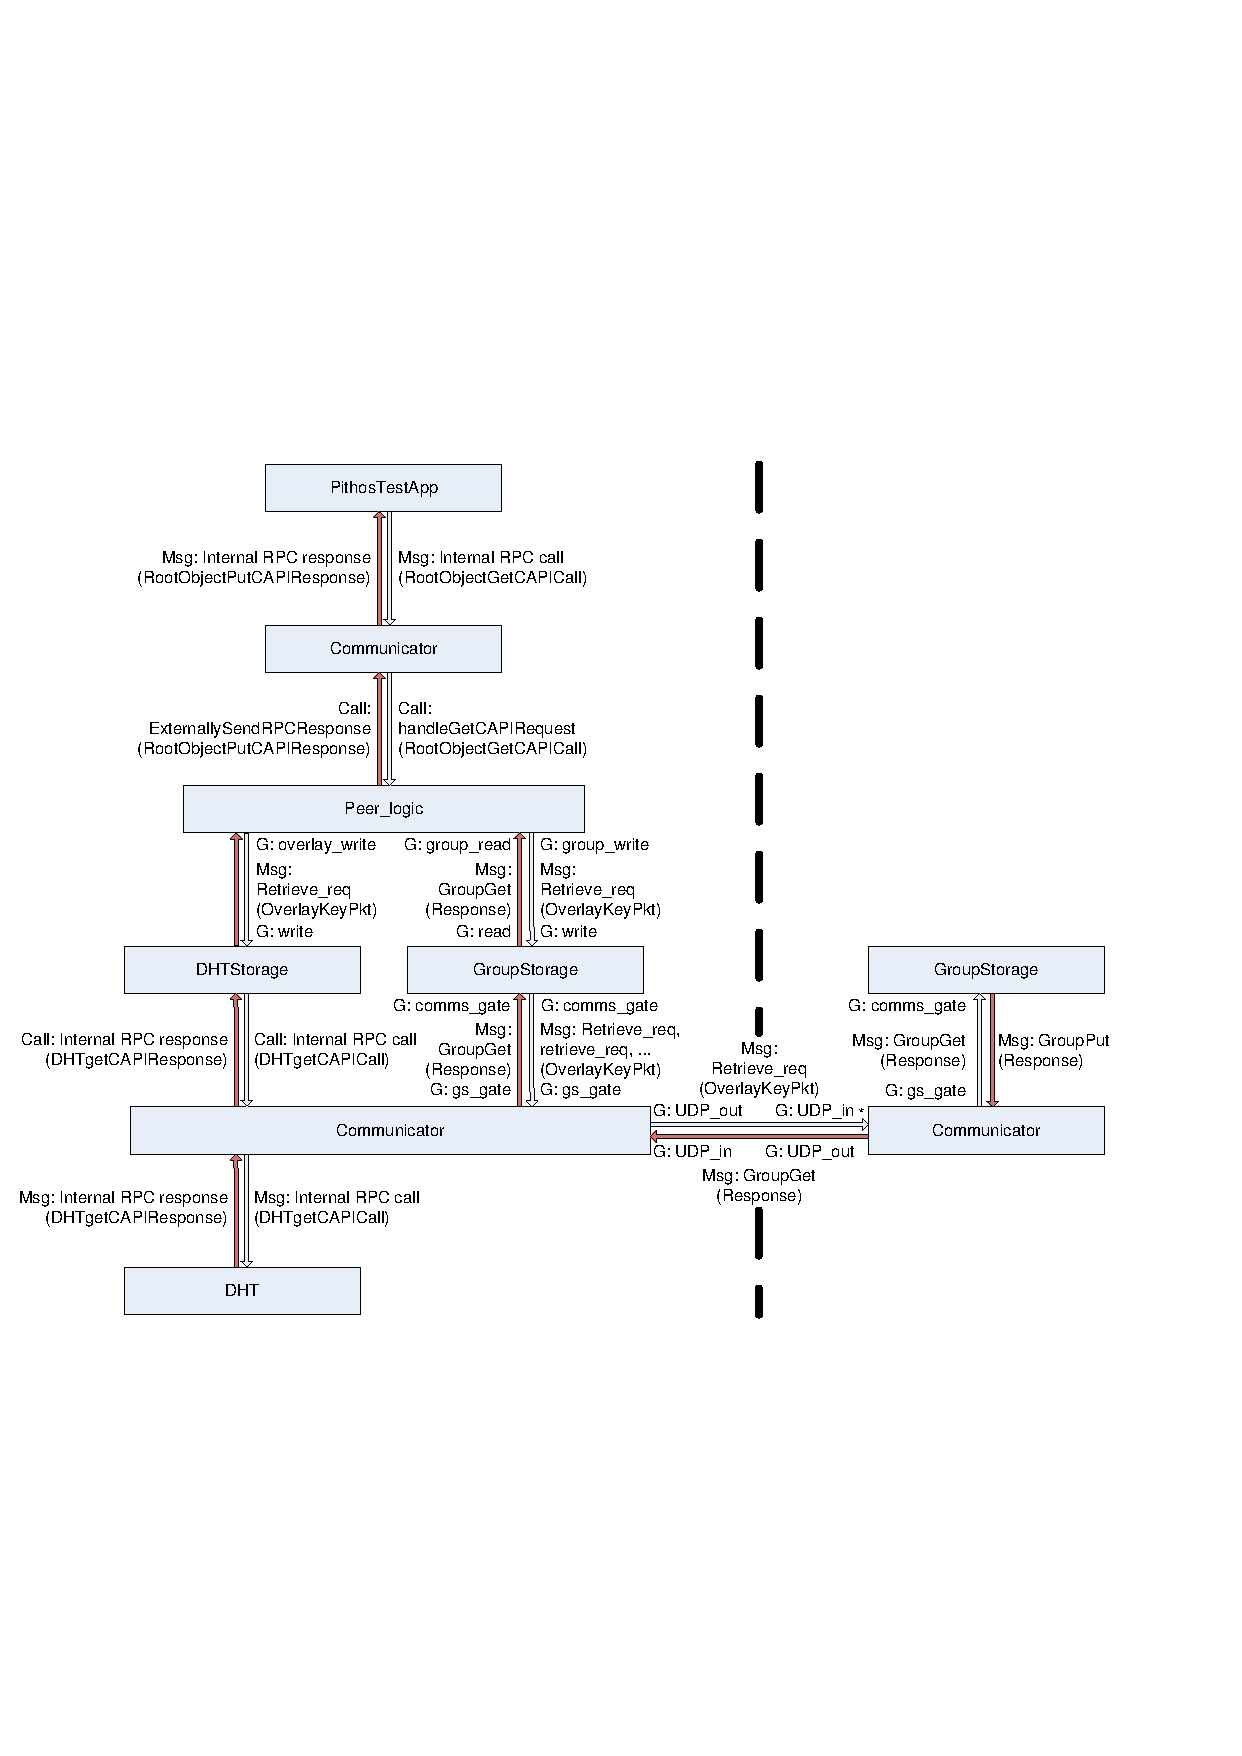
\includegraphics[clip=true, viewport=3mm 73mm 189mm 219mm, width=\columnwidth]{Pithos_msg_flows_retrieve}
 \caption{Pithos message flow as a response to a retrieve request}
 \label{fig_pithos_msg_flow_retrieve}
\end{figure}

    Group storage first checks whether the object that was requested exists within the group by checking its group ledger. This is required, because the PithosTestApp might require an object that is stored in another group. The out of group request will then only fulfilled by the DHT storage module. If the object is housed in the group storage's local store, the object is sent up to the peer logic module. If the object is found in the group ledger, but not on the peer where the requests originated from, a peer has to be selected to retrieve the object from. The number of peers selected depends on a parameter in the configuration file. More requests sent in parallel will improve the probability of the request succeeding as well as reduce the time it takes to serve the request.

    Retrieve requests mainly fail because of nodes leaving a group. If a node leaves before it can serve an object, the object request fails. If multiple requests are sent, it improves the chances of contacting a node that is not about to leave, which improves the probability of retrieval success. More requests also improve lookup times, since some peers might be geographically closer to the requesting peer, thereby possessing a lower latency. Sending multiple requests improves the chances of contacting a peer that is closer, which improves the responsiveness of the systems. The disadvantage of multiple requests is the extra bandwidth required, both in sending the requests and in the duplicate objects that will be returned. The effect of multiple requests on system reliability, responsiveness and overhead will be evaluated in Chapter \ref{chp:EVALUATION}.

    A request is delivered to the destination peer, which forwards the request to the group storage module. The group storage module retrieves the object from its local storage, attaches it to a response message and sends that response to the source peer. The response is forwarded to the group storage module, which collects statistics before passing it on to the peer logic module. After the peer logic module has received a sufficient number of responses, it informs the higher layer of either a successful or failed retrieval. The object itself is attached to a successful request response.

    Again, two types of retrieval have been implemented: ``fast'' and ``safe''. A fast retrieval sends the first successful response, and therefore, the first successful object, to the higher layer. It replies with failure if all requests failed. The safe retrieval request is more resistent to malicious nodes. For safe retrieval, the peer logic waits for a specified number of responses. It then compares all objects received from successful responses and sends an object to the higher layer that had the most matches when compared. This is to counter a malicious peer that might have altered some of the objects before sending them. The reliability benefit with this scheme in the presence of malicious nodes will be shown in Section \ref{reliability_compare_retrieval}.

    \subsubsection{Modifying data}
    \label{modify_implementation}

    Modifying data is similar to storing data. A request to modify a specific object is received from the PithosTestApp. The request specifies the object ID, the parameter that has to be modified and the new value of the parameter. The update is delivered to the peer logic, where the modify request is sent to DHT and group storage. The Oversim DHT handles the modify request and responds with success or failure. Group storage received the modify request and checks the group ledger whether the object exists within the group. If the object does not exist in the group, it is only modified in the overlay. To keep track of modified objects, each object has a version number that is incremented every time an object is modified. This allows retrieve requests to select the object with the latest version number to be sent to the higher layer.

    If the object exists within the group, all peers that contain the object are identified from the group ledger and modify requests are sent to them. The modify request will be sent to the destination group storage module where the object in the local store is updated and its version number incremented. If a retrieve request receives objects with multiple version numbers, it selects the set of objects with the latest version number for ``fast'' or ``safe'' comparison.

    \subsubsection{Tracking requests}
    \label{pending_rpcs_implementation}

    When sending a request to a destination peer, the destination peer might leave the group before it can receive the request or respond to it. No response will, therefore, be sent to the source peer, which might cause come requests to remain unresolved. For example, if safe storage is used and the system waits for all responses before informing the higher layer of the request status, the higher layer will never be informed if a destination node has left. A mechanism is required to handle nodes leaving the group.

    The solution is for super peer logic, peer logic and DHT modules track all requests sent and link every outstanding request with a timeout. Every one of those modules contains a pending requests list. Each pending request is uniquely identified by the RPC ID received from PithosTestApp. Each pending request from the higher layer usually generates multiple messages to DHT storage, and multiple nodes in the group via group storage.

    Every request sent out by the DHT storage or group storage modules contain the RPC ID of the original request from PithosTestApp. The RPC ID is copied into the response at the destination location. This allows every response to be linked to the original request that generated it. When a response is received from a peer, the pending request for the RPC ID for that peer is removed from the pending requests list.

    Every pending request is also linked to a timeout. If the timeout expires, the pending request is removed and a failure response is generated and sent to the higher layer. This mechanisms ensures that all requests will always receive all expected responses. It also handled peers leaving groups.

    It is accepted that this mechanism may cause false negatives if there is a delay due to congestion in the network. This situation can be avoided by making the timeout sufficiently long.

    \subsubsection{Group migration}
    \label{group_migration_implementation}

    Users will constantly being moving in the virtual environment, leading to changes in position. These position changes may lead to users moving from one group to another. It imperative that all objects stored in Pithos remain available even with users traversing groups. To simulate the effect that user movement will have on objects stored in Pithos, PithosTestApp is designed to generate position updates.

    PithosTestApp simulates a user moving around in a virtual world. This is done by having PithosTestApp generate a new random position chosen in the same way as when a node joined a group: by selected x and y coordinates in a uniformly random fashion. A position update timer determines when a node's position should change. It is accepted that the movement this scheme will generate will not match the way users move in a virtual world. Modelling accurate user movement is, however, not important for the Pithos simulation. Storing and retrieving objects in Pithos only depends on which group a user occupies and how Pithos handles a user that moves to another group. The order in which a user might enter groups or, in fact, the specific group that a user moves to, is not important. All that is important is how objects are handled when any group migration occurs.

    When a new position is generated by PithosTestApp, this is sent to the group storage module. The group storage module queries the directory server with the new position, using the same mechanism described for joining a group in Section \ref{network_join_implementation}. Group storage receives a super peer address from the directory server, if this address is different from the address of the currently known super peer, group storage initiates group migration.

    Group migration involves informing the group that the peer is leaving, clearing all statistics and initiating the group join mechanism. Informing the group that the peer is leaving ensures that this peer will not be picked for any storage or retrieval requests, while the group is unaware that the peer has left. If this is not done, the group will only know that a peer has left after a timeout for a request to the peer expires. This reduces request success rates.

    \subsubsection{Group consistency}
    \label{group_migration_implementation}

    With peers constantly joining and leaving the network and transferring between groups, an issue that arises is group consistency. It is important that all peers within a group share the same view of that group. If this is not the case, some peers might never be chosen to store data and this will decrease the fairness in the system. Another reason is that for the sake of scalability, peers do not service requests from peers outside of their groups. Group inconsistencies might also lead to nodes becoming isolated from any group, which basically disconnects that node from the P2P network.
    
The initial approach to achieve group consistency was to have every peer inform all other peers when it was moving from one group to another. If a peer was removed from the network due to churn, another peer has to discover that the peer has left. This was done when requests timed out. If a request times out, the peer making the request informs the group of the peer that left.
    
    \begin{figure}[htbp]
 \centering
 \includegraphics[clip=true, viewport=0mm 0mm 460mm 212mm, width=\columnwidth]{gc_first}
 \caption{Group consistency before any improvements}
 \label{fig_gc_first}
\end{figure}
%
Figure \ref{fig_gc_first} shows the perceived group size of every node in the group for the initial group consistency scheme. From approximately 2925 s, a new peer joins the group and reports the group size is eight, when all other peers report the group size as seven. Initially, it might appear that the group peers are not aware of the new peer that has joined the group. This is not the case. What is in fact happening is that a peer has left, just as the new peer joined. All group peers recorded the peer leaving and the new peer joining.

The issue has to do with how how objects are handled in group storage. When a new peer joins the group, it starts to generate objects. The group super peer sends a joining peer a list of group peers. After this occurs, the group peers are informed of the new peer. A peer joining a group can immediately start to create objects for group storage. Situations arise where a new object is sent to a group peer for storage, before the group peer is aware of the peer that generated the object. The solution was to assume that an object was generated by a valid peer and to add any unknown peer information contained in an object store request to the peers list in the group ledger.

The group inconsistency issue then arises, because the peer informing the group of the peer that left, is not yet aware of the peer that joined. Only after the super peer informs the group peers of the new peer is everyone aware of it. When the super peer sends the joining peer the group peer list, it has not yet been informed of the peer leaving. The new peer, therefore, also thinks that the peer that left is still present in the group.

This transition issue was solved by the super peer storing the information of the last peer that left. Every time a new peer join, the super peer also informs the joining peer of the last peer that left. This allows the joining peer to ignore any latent object add messages received from the leaving peer.

    \begin{figure}[htbp]
 \centering
 \includegraphics[clip=true, viewport=0mm 0mm 455mm 212mm, width=\columnwidth]{gc_middle}
 \caption{Group consistency with starvation}
 \label{fig_gc_middle}
\end{figure}
%
This created the issue shown in Figure \ref{fig_gc_middle}, where a peer will believe that another peer has left. The group will be informed of the peer that supposedly left, but is actually still present in the group.

    \begin{figure}[htbp]
 \centering
 \includegraphics[clip=true, viewport=0mm 0mm 430mm 180mm, width=\columnwidth]{gc_final}
 \caption{Group consistency after all improvements}
 \label{fig_gc_final}
\end{figure}

    \subsubsection{Object repair}
    \label{object_repair_implementation}

    \subsubsection{Object verification}
    \label{object_verification_implementation}

\section{PithosTestApp implementation}
\label{pithostestapp}

\section{Bandwidth requirements (overhead)}
    %Mention something about low bandwidth links and how that influences timeout and what extra mechanisms were required.
    %Check how this increases with increased network sizes and varying levels of network churn.
